\documentclass[12pt, a4paper, oneside]{ctexart}
\usepackage{amsmath, amsthm, amssymb, bm, color, graphicx, geometry, mathrsfs,extarrows, braket, booktabs, array}
\usepackage[colorlinks,linkcolor=red,anchorcolor=blue,citecolor=blue,urlcolor=blue,menucolor=black]{hyperref}
\setmainfont{Times New Roman}  % 设置英文字体
\setsansfont{Calibri}
\setmonofont{Consolas}

\linespread{1.4}
%\geometry{left=2.54cm,right=2.54cm,top=3.18cm,bottom=3.18cm}
\geometry{left=1.84cm,right=1.84cm,top=2.18cm,bottom=2.18cm}
\newenvironment{problem}{\par\noindent\textbf{题目. }}{\bigskip\par}
\newenvironment{solution}{\par\noindent\textbf{解答. }}{\bigskip\par}
\newenvironment{note}{\par\noindent\textbf{注记. }}{\bigskip\par}

%%%% 图片相对路径 %%%%
\graphicspath{{figure/}} % 当前目录下的figure文件夹, {../figure/}则是父目录的figure文件夹

\everymath{\displaystyle} % 默认全部行间公式
\DeclareMathOperator*\uplim{\overline{lim}} % 定义上极限 \uplim_{}
\DeclareMathOperator*\lowlim{\underline{lim}} % 定义下极限 \lowlim_{}
\let\leq=\leqslant % 将全部leq变为leqslant
\let\geq=\geqslant % geq同理

% 一些宏定义
\def\bd{\boldsymbol}        % 加粗(向量) boldsymbol
\def\disp{\displaystyle}    % 使用行间公式 displaystyle(默认)
\def\tsty{\textstyle}       % 使用行内公式 textstyle
\def\sign{\text{sign}}      % sign function
\def\wtd{\widetilde}        % 宽波浪线 widetilde
\def\R{\mathbb{R}}          % Real number
\def\N{\mathbb{N}}          % Natural number
\def\Z{\mathbb{Z}}          % Integer number
\def\C{\mathbb{C}}          % Complex number
\def\d{\mathrm{d}}          % differential operator
\def\e{\mathrm{e}}          % Euler's number
\def\i{\mathrm{i}}          % imaginary number
\def\re{\mathrm{Re}}        % Real part
\def\im{\mathrm{Im}}        % Imaginary part
\def\res{\mathrm{Res}}      % Residue
\def\L{\mathcal{L}}         % Loss function
\def\wdh{\widehat}          % 宽帽子 widehat
\def\ol{\overline}          % 上横线 overline
\def\ul{\underline}         % 下横线 underline
\def\diam{\text{diam }}      % 直径 diameter
\def\add{\vspace{1ex}}      % 增加行间距
\def\del{\vspace{-1.5ex}}   % 减少行间距

% 基本信息
\newcommand{\RQ}{\today} % 日期
\newcommand{\km}{泛函分析} % 科目
\newcommand{\bj}{强基数学002} % 班级
\newcommand{\xm}{吴天阳} % 姓名
\newcommand{\xh}{2204210460} % 学号

\begin{document}

%\pagestyle{empty}
\pagestyle{plain}
\vspace*{-15ex}
\centerline{\begin{tabular}{*5{c}}
    \parbox[t]{0.25\linewidth}{\begin{center}\textbf{日期}\\ \large \textcolor{blue}{\RQ}\end{center}} 
    & \parbox[t]{0.2\linewidth}{\begin{center}\textbf{科目}\\ \large \textcolor{blue}{\km}\end{center}}
    & \parbox[t]{0.2\linewidth}{\begin{center}\textbf{班级}\\ \large \textcolor{blue}{\bj}\end{center}}
    & \parbox[t]{0.1\linewidth}{\begin{center}\textbf{姓名}\\ \large \textcolor{blue}{\xm}\end{center}}
    & \parbox[t]{0.15\linewidth}{\begin{center}\textbf{学号}\\ \large \textcolor{blue}{\xh}\end{center}} \\ \hline
\end{tabular}}
\vspace*{4ex}

% 正文部分
\paragraph*{1.}分别证明$\rho_1(x, y) = \max_{a\leq t\leq b}|x(t) - y(t)|,\ \rho_2(x, y)=\int_a^b|x(t)-y(t)|\,\d t$是$C[a, b]$中的度量.
\begin{proof}
    任取$x, y, z\in C[a, b]$.

    (正定性)由于$|x(t) - y(t)|\geq 0$,则$\rho_1(x, y) = \max_{a\leq t\leq b}|x(t)-y(t)|\geq 0$.
    
    若$\rho_1(x, y) = 0$,则$|x(t)-y(t)|\leq \max_{a\leq t\leq b}|x(t)-y(t)| = 0$,则$x(t) = y(t)$;反之,当$x(t)=y(t)$,则$\rho_1(x, y) = \max_{a\leq t\leq b}0 = 0$.
    
    设$\pi:a=a_1<a_2<\cdots<a_n=b$为$[a,b]$上的一个划分,$\Delta\pi = \max_{(a_i, a_{i+1})\in \pi}a_{i+1}-a_i$,则
    \begin{equation*}
        \rho_2(x,y)=\int_a^b|x(t)-y(t)|\,\d t = \lim_{\Delta\pi\to0}\sum_{(a_i,a_{i+1})\in\pi}|x(\xi_i)-y(\xi_i)|(a_{i+1}-a_i)
    \end{equation*}
    其中$\xi_i\in(a_i,a_{i+1})$. 由于$|\cdot|$和$(a_{i+1}-a_i)$均大于等于$0$,则$\rho_2(x,y)\geq 0$.
    
    若$\rho_2(x, y)=  0$,则 $\int_a^b|x(t)- y(t)|\,\d t = 0$则$|x(t)-y(t)|$在$[a,b]$上几乎处处为$0$,又由于连续性可知处处为$0$,即$x(t)=y(t)$;反之,当$x(t) = y(t)$,则$\rho_2(x, y) = \int_a^b0\,\d t = 0$.

    (对称性)\del
    \begin{align*}
        \rho_1(x, y) =&\ \max_{a\leq t\leq b}|x(t)-y(t)| = \max_{a\leq t\leq b}|y(t)-x(t)| = \rho_1(y, x)\\
        \rho_2(x, y) =&\ \int_a^b|x(t)-y(t)|\,\d t = \int_a^b|y(t)-x(t)|\,\d t=\rho_2(y,x)
    \end{align*}

    (三角不等式)\del
    \begin{align*}
        \rho_1(x, y)=&\ \max_{a\leq t\leq b}|x(t)-y(t)|\leq\max_{a\leq t\leq b}(|x(t)-z(t)|+|z(t)-y(t)|) \\
        \leq&\ \max_{a\leq t\leq b}|x(t)-z(t)|+\max_{a\leq t\leq b}|z(t)-y(t)| \leq \rho_1(x, z)+\rho_1(y, z)\\
        \rho_2(x, y) =&\ \int_a^b|x(t)-y(t)|\,\d t\leq \int_a^b(|x(t)-z(t)|+|z(t)-y(t)|)\,\d t\\
        \leq&\ \int_a^b|x(t)-z(t)|\,\d t+\int_a^b|z(t)-y(t)|\,\d t = \rho_2(x, z) + \rho_2(y, z)
    \end{align*}
\end{proof}

\paragraph*{2.} 证明$\rho(x, y) = \frac{|x-y|}{1+|x-y|}$是$\R$中的度量.
\begin{proof}
    (正定性)由于$|x-y|,1+|x-y|\geq 0$,则$\rho(x, y)\geq 0$.
    
    $\rho(x, y) = 0\iff |x-y| = 0\iff x=y$.

    (交换性)由于$|x-y| = |y-x|$,则$\rho(x, y) = \rho(y, x)$.

    (三角不等式)
    \begin{align*}
        \rho(x, y) =&\ \frac{|x-y|}{1+|x-y|} = \frac{1}{\frac{1}{|x-y|}+1}\leq \frac{1}{\frac{1}{|x-z|+|z-y|}+1}=\frac{|x-z|+|z-y|}{1+|x-z|+|z-y|}\\
        \leq&\ \frac{|x-z|}{1+|x-z|}+\frac{|y-z|}{1+|y-z|}= \rho(x, z) + \rho(y, z)
    \end{align*}
\end{proof}

\paragraph*{3.}$S[a,b]$表示$[a,b]$上几乎处处有取值的可测函数全体,证明$\rho(f, g) = \int_a^b\frac{|f-g|}{1+|f-g|}\,\d \mu$为其上的一个度量.
\begin{proof}
    由第\textbf{2}题可知,$\frac{|f-g|}{1+|f-g|}$满足正定性、交换性和三角不等式,则$\rho(f,g)\geq 0,\rho(f,g) = \rho(g, f)$,当$\rho(f,g)=0$时,$f,g$几乎处处相等. 由积分的线性性可知
    \begin{align*}
        \rho(f,g)=&\ \int_a^b\frac{f-g}{1+|f-g|}\,\d \mu \leq \int_a^b\left(\frac{|f-h|}{1+|f-h|}+\frac{|g-h|}{1+|g-h|}\right)\,\d\mu\\
        =&\ \int_a^b\frac{|f-h|}{1+|f-h|}\,\d\mu+\int_a^b\frac{|g-h|}{1+|g-h|}\,\d\mu=\rho(f,h)+\rho(g,h)
    \end{align*}
\end{proof}

\paragraph*{4.}证明$\rho(f,g)=\left(\int_a^b|f-g|^p\,\d x\right)^{1/p}$是$L^p[a, b],\ (1\leq p\leq \infty)$上的一个度量.
\begin{proof}
    $\rho(f,g) = ||f-g||_p$,其中$||f-g||_p$为$f-g$的p-范数.
    
    (正定性)由于p-范数满足正定性,则$\rho(f,g)\geq 0$,当$\rho(f,g)=0\iff f=g\quad a.e.$
    
    (交换性)由于$|f-g|^p = |g-f|^p$,则$\rho(f,g) = \rho(g,f)$. 

    (三角不等式)由Minkowski不等式知,$||f-g||_p\leq ||f-h||_p+||g-h||_p$,于是$\rho(f,g)\leq \rho(f,h)+\rho(g,h)$.
\end{proof}

\paragraph*{5.}设$(X,\rho)$为度量空间,$A\subset X$,则$A$是闭集$\iff$$A$包含$A$中所有收敛列的极限点.
\begin{proof}
    “$\Rightarrow$”:当$A$是闭集,则$A^c$为开集. $\forall x\in A^c$,$\exists r>0$使得$B(x, r)\subset A^c$,任取收敛列$\{x_n\}\subset A,\ x_n\to x$. 假设$x\notin A$,则$x\in A^c$. 由于$\rho(x_n,x)\to 0$,则存在$N\in\mathbb{N}$使得$\forall n\geq N$有$\rho(x_n, x) < r$,则$x_n\in B(x, r)\Rightarrow x_n\in A^c$与$x_n\in A$矛盾,故$x\in A$.

    “$\Leftarrow$”:$\forall x\in A^c$,假设对$\forall r>0$都有$B(x, r)\cap A\neq \varnothing$,则$\exists \{x_n\}\subset A$且$x_n\to x$,由原命题条件可知$x\in A$,与$x\in A^c$矛盾,则$\exists r >0$使得$B(x,r)\cap A=\varnothing$,则$B(x,r)\subset A^c$,故$A^c$为开集,即$A$为闭集.
\end{proof}

\paragraph*{6.}设$(X,\rho)$为度量空间,$A\subset X$,定义$\diam A:=\sup_{x,y\in A}\rho(x, y)$,证明:$\diam A=\diam\bar{A}$.
\begin{proof}
    只需证$\sup_{x,y\in A}\rho(x, y) = \sup_{x,y\in \bar{A}}\rho(x, y)$.
    
    设$\sup_{x,y\in\bar{A}}\rho(x,y)=M$,由于$\bar{A} = A\cup A'$,则$\sup_{x,y\in A}\rho(x, y)\leq M$.
    
    $\forall \varepsilon >0$,$\exists x, y\in\bar{A}$使得$\rho(x, y) > M-\varepsilon$. 于是存在$\{x_n\},\{y_n\}\subset A$使得$x_n\to x, y_n\to y$. 则$\exists N\in\N$使得$\forall n\geq N$有
    \begin{equation*}
        \rho(x, x_n)\leq \varepsilon,\quad \rho(y, y_n)\leq \varepsilon,\quad (n\geq N)
    \end{equation*}
    于是
    \begin{align*}
        &\ M-\varepsilon < \rho(x, y)\leq \rho(x,x_n)+\rho(x_n,y_n)+\rho(y_n, y)\leq 2\varepsilon + \sup_{x,y\in A}\rho(x, y)\\
        \Rightarrow&\ M-3\varepsilon< \sup_{x,y\in A}\rho(x, y)\leq M\quad (n\geq N)
    \end{align*}
    由$\varepsilon$的任意性知$\sup_{x, y\in A}\rho(x, y) = M$,即$\diam A = \diam \bar{A}$.
\end{proof}

\paragraph*{7.}设$(X,\rho)$为度量空间,$E\subset X$,则$E$是疏集$\iff$$\forall \ol{B(x, r)} = \{z\in X:\rho(z, x)\leq r\}$必存在开球$B(x',r')\subset B(x, r)$使得$\ol{B(x',r')}\cap \bar{E}=\varnothing$.
\begin{proof}
    “$\Rightarrow$”:由于$\bar{E}$无内点,则$\forall x\in \bar{E}$,$\forall \varepsilon > 0$有$B(x, \varepsilon)\not\subset \bar{E}$,即$B(x,\varepsilon) - \bar{E}\neq\varnothing$,且$B(x,\varepsilon)-\bar{E} = B(x,\varepsilon)\cap \bar{E}^c$为开集.

    取$x'\in B(x,\varepsilon) - \bar{E}$,则$\exists \delta  > 0$使得$B(x',\delta)\subset B(x,\varepsilon)-\bar{E}$,则$B(x',\delta)\cap \bar{E} = \varnothing\Rightarrow \ol{B(x',\delta/2)}\cap \bar{E} = \varnothing$.
    
    “$\Leftarrow$”:假设$\bar{E}$有内点,则$\exists x\in \bar{E}$,$\exists \varepsilon > 0$,使得$B(x, \varepsilon) \subset \bar{E}$,则$\forall B(x',r')\subset B(x, \varepsilon)$,$B(x',r')\cap \bar{E}\neq\varnothing$,与原命题条件矛盾,则$\bar{E}$无内点.
\end{proof}

% 下面给一些功能的写法
\iffalse
% 图片模板
\centerline{
    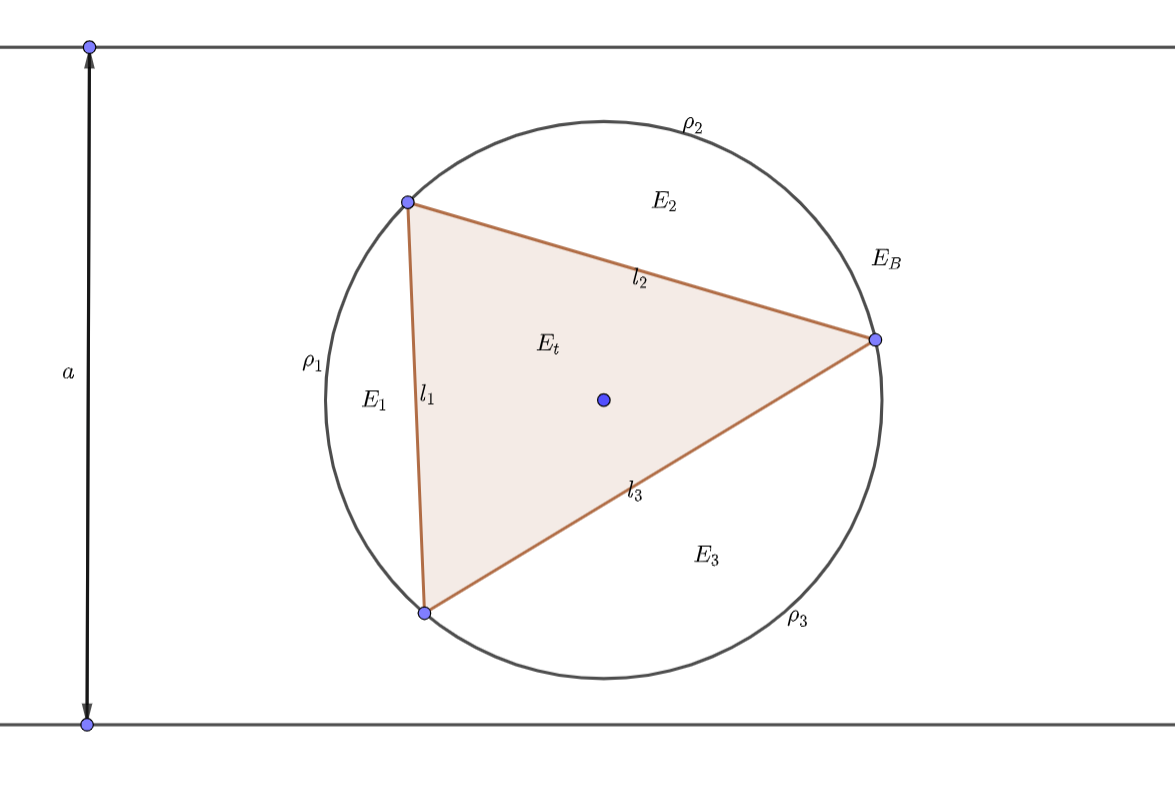
\includegraphics[width=0.8\textwidth]{figure.png}
}
% 表格模板
\renewcommand\arraystretch{0.8} % 设置表格高度为原来的0.8倍
\begin{table}[!htbp] % table标准
    \centering % 表格居中
    \begin{tabular}{p{1cm}<{\centering}p{1cm}<{\centering}p{3cm}<{\centering}p{5cm}<{\centering}} % 设置表格宽度
    %\begin{tabular}{cccc}
        \toprule
        $x_i$ & $f[x_1]$ & $f[x_i,x_{i+1}]$ & $f[x_i,x_{i+1},x_{i+2}]$ \\
        \midrule
        $x_0$ & $f(x_0)$ &                  &                          \\
        $x_0$ & $f(x_0)$ & $f'(x_0)$        &                          \\
        $x_0$ & $f(x_1)$ & $\frac{f(x_1)-f(x_0)}{x_1-x_0}$ & $\frac{f(x_1)-f(x_0)}{(x_1-x_0)^2}-\frac{f'(x_0)}{x_1-x_0}$\\
        \bottomrule
    \end{tabular}
\end{table}

\def\Log{\text{Log}} % 一个简单的宏定义
$\Log$ % 调用方法
\fi

\end{document}